\documentclass[conference]{IEEEtran}
\IEEEoverridecommandlockouts

\usepackage{tikz}
\usetikzlibrary{arrows.meta, positioning, fit, backgrounds, shapes.geometric, calc}
\usepackage{amsmath,amssymb,amsfonts}
\usepackage{algorithmic}
\usepackage{graphicx}
\usepackage{textcomp}
\usepackage{xcolor}
\usepackage{listings}
\usepackage{booktabs}
\usepackage{multirow}
\usepackage{subcaption}
\usepackage{pgfplots}
\pgfplotsset{compat=1.18}
\usepackage{enumitem}
\usepackage{url}

\lstset{
    basicstyle=\ttfamily\small,
    keywordstyle=\color{blue},
    commentstyle=\color{gray},
    stringstyle=\color{red},
    showstringspaces=false,
    breaklines=true,
    frame=single,
    numbers=left,
    numberstyle=\tiny\color{gray},
    captionpos=b
}

\usepackage[backend=biber]{biblatex}
\addbibresource{paper.bib}

\graphicspath{{experiments/figures/}}

\begin{document}

\title{QLego: Cross-Compiler Pass Composition for\\Quantum Circuit Optimization}

\author{
  \IEEEauthorblockN{Abhishek Shringi}
  \IEEEauthorblockA{\textit{Department of Computer Science}\\
    University at Albany, SUNY\\
    Albany, NY, USA\\
    ashringi@albany.edu}
}

\maketitle

%===================================================================
\begin{abstract}
%===================================================================
Quantum compilation transforms abstract quantum algorithms into executable instructions for constrained, noisy hardware through a sequence of optimization passes including qubit mapping, routing, and gate optimization.
Existing quantum SDKs each implement proprietary, fixed compilation pipelines, preventing systematic composition of best-in-class passes across toolchains.
We introduce \textbf{QLego}, a modular cross-compiler framework that decomposes quantum compilation into discrete, interchangeable passes and enables hybrid pipelines combining algorithms from Qiskit, TKet, BQSKit, and Cirq.
Each plugin executes in an isolated virtual environment, eliminating dependency conflicts while maintaining seamless communication through OpenQASM serialization and a unified hardware abstraction.

Using QLego, we conduct a comprehensive case study of over \textbf{5,000} compilation configurations across 10 benchmark circuit families, 14 layout strategies, 11 routing strategies, and 32 optimization passes on two hardware topologies (65-qubit heavy-hex and all-to-all connectivity).
Our study tests three hypotheses and yields the following findings:
(i)~the optimal pass sequence is strongly dependent on circuit structure, with no single SDK dominating across all circuit families;
(ii)~cross-SDK optimization passes are \textit{complementary}---after one SDK's optimizer converges, a different SDK extracts up to \textbf{68\%} additional depth reduction, with 5 of 6 inter-SDK orderings yielding positive residual improvement;
(iii)~optimization passes can exhibit \textit{destructive interference}, where adding a correct pass increases circuit depth---4.5\% of incremental pass applications increase depth, and three orderings of the same six passes produce divergent quality trajectories;
and (iv)~optimization pass rankings are moderately to strongly correlated across hardware topologies (median Spearman $\rho = 0.926$, range 0.613--0.999), yet the best pass changes between topologies in 17 of 19 tested circuit--scale pairs (89\%), confirming topology-dependent ordering effects.
These results demonstrate that cross-framework pass composition is not merely convenient but reveals fundamental properties of quantum optimization landscapes, establishing QLego as infrastructure for AI-driven compiler research.

\end{abstract}

\begin{IEEEkeywords}
quantum compilation, cross-compiler optimization, pass composition, circuit benchmarking, NISQ
\end{IEEEkeywords}

%===================================================================
\section{Introduction}
\label{sec:introduction}
%===================================================================

Quantum computing promises to solve problems intractable for classical machines, yet realizing this potential depends critically on the software that compiles high-level algorithms into executable instructions for constrained, noisy hardware~\cite{preskill2018quantum}.
This compilation process involves a sequence of NP-Hard optimization passes---qubit mapping, routing, gate unrolling, and circuit optimization---each requiring significant trade-offs between resource demands and output quality~\cite{siraichi2018qubit}.

A growing ecosystem of quantum software development kits (SDKs) has emerged to address this challenge.
Qiskit~\cite{qiskit}, TKet~\cite{sivarajah2020tket}, BQSKit~\cite{patel2022bqskit}, and Cirq each implement their own compilation pipelines, employing different algorithmic strategies for the same underlying problems.
Benchmarking suites such as Benchpress~\cite{benchpress} and MQT Bench~\cite{quetschlich2023mqtbench} have enabled systematic \textit{comparison} of these compilers' outputs.
However, a fundamental limitation persists: these tools compare the final output of different compilers but do not enable the \textit{composition} of individual passes across toolchains.
A researcher who discovers that Qiskit's SABRE mapper excels for one circuit structure while TKet's peephole optimizer yields superior depth for another has no systematic way to combine these best-in-class components.

This limitation is not merely an engineering inconvenience.
It obscures a fundamental scientific question: \textit{are the optimization strategies employed by different SDKs complementary or redundant?}
If complementary---that is, if one SDK's optimizer can extract further reductions after another SDK's optimizer has fully converged---then the current practice of single-SDK compilation is provably leaving performance on the table.
Furthermore, the classical compiler literature has long recognized the \textbf{phase ordering problem}: the optimal sequence of individually correct optimization passes depends on the input program and cannot be determined a priori~\cite{click1995combining}.
Whether this phenomenon manifests in quantum compilation, and whether it extends \textit{across} compiler boundaries, remains empirically uncharacterized.

To address these gaps, we introduce \textbf{QLego}, a modular cross-compiler framework for quantum circuit optimization.
QLego decomposes the compilation flow into discrete, interchangeable passes and provides a unified interface to integrate algorithms from diverse SDKs, with each plugin executing in an isolated virtual environment to prevent dependency conflicts.
This design enables the creation of hybrid pipelines that combine, for example, a layout pass from BQSKit, a router from TKet, and an optimizer from Qiskit.

Using QLego, we conduct a systematic case study comprising over 5,000 compilation configurations to test three hypotheses about the structure of the quantum compilation optimization landscape:

\begin{enumerate}[label=\textbf{H\arabic*},leftmargin=*]
    \item \textbf{Domain Specialization.} The optimal pass sequence depends on circuit structure; no single SDK or pass universally dominates.
    \item \textbf{Cross-SDK Complementarity.} Optimization passes from different SDKs are complementary: after one SDK's optimizer converges to a fixed point, a different SDK can extract additional reductions.
    \item \textbf{Destructive Interference.} Adding a correct optimization pass to a pipeline can \textit{increase} circuit depth or gate count, and this effect is ordering-dependent.
\end{enumerate}

Our contributions are as follows.
First, we present the QLego framework: a plugin-based, dependency-isolated cross-compiler architecture enabling modular hybrid quantum compilation pipelines (\S\ref{sec:framework}).
Second, we validate that QLego's isolation model introduces zero quality degradation (\S\ref{sec:validation}).
Third, through a comprehensive case study on two hardware topologies across 10 circuit families, we provide the first empirical evidence for all three hypotheses (\S\ref{sec:casestudy}--\S\ref{sec:results}).
Fourth, we demonstrate that hardware topology independently affects optimal pass ordering, not just pass selection (\S\ref{sec:topology}).

%===================================================================
\section{Background}
\label{sec:background}
%===================================================================

\subsection{Quantum Circuit Compilation}

The execution of quantum algorithms on physical hardware requires a compilation process that bridges abstract circuit descriptions and device-specific constraints.
The primary objectives are to respect hardware limitations while minimizing susceptibility to noise and decoherence~\cite{preskill2018quantum, cowtan2019phase}.
The compilation workflow consists of the following core stages:

\textbf{Decomposition.}
Complex, high-level operations are decomposed into a basis set of elementary gates (typically single-qubit rotations and CNOT gates).

\textbf{Qubit Mapping (Layout).}
Logical qubits are assigned to physical qubits on the device, subject to its connectivity constraints~\cite{siraichi2018qubit}.
An effective layout minimizes subsequent routing overhead by placing interacting qubits on adjacent physical locations.

\textbf{Routing.}
Two-qubit gates between non-adjacent physical qubits are resolved by inserting SWAP operations, each typically decomposed into three CNOTs~\cite{li2019tackling, cowtan2019phase}.
Minimizing SWAP insertion is critical, as each additional CNOT increases circuit depth and accumulated error.

\textbf{Translation.}
Gates are translated into the hardware's native gate set (e.g., $\sqrt{X}$, $R_Z$, CNOT).

\textbf{Optimization.}
Peephole optimizations, commutation-based cancellations, and resynthesis techniques eliminate redundant operations and reduce overall gate count and depth.

The layout and routing problems are NP-Hard~\cite{itoko2020optimization, wille2019mapping}.
Beyond algorithmic complexity, NISQ compilation must contend with hardware \textit{non-stationarity}: qubit relaxation times ($T_1$, $T_2$) and gate error rates fluctuate over time~\cite{tannu2019not}, necessitating adaptive compilation strategies.

\subsection{The Phase Ordering Problem}

A fundamental challenge in compiler design is the \textbf{phase ordering problem}: determining the optimal sequence of individually correct optimization passes~\cite{click1995combining}.
Since each pass can expose or inhibit opportunities for subsequent passes, applying pass $A$ before $B$ can produce a different result than $B$ before $A$, even when both are independently valid transformations.

In quantum compilation, this manifests acutely.
A noise-reducing optimization applied before routing may increase final gate count, because routing reintroduces redundancies.
Conversely, a router that minimizes SWAP count at the expense of circuit topology may prevent subsequent peephole optimizers from finding cancellation opportunities.
The standard approach of using a fixed, heuristically-designed pass order (as employed by all major SDKs) is provably suboptimal for general circuits.

This motivates two complementary approaches: exhaustive enumeration (enabled by a framework like QLego) reveals the performance landscape empirically, while machine learning predicts good orderings from circuit features~\cite{quetschlich2024mqtpredictor, mills2026rl}.
QLego provides infrastructure for both.


%===================================================================
\section{Related Work}
\label{sec:relatedwork}
%===================================================================

\subsection{Quantum Compiler Frameworks}

\textbf{Qiskit}~\cite{qiskit} provides a rich transpiler with algorithmic choices for mapping (TrivialLayout, DenseLayout, SabreLayout) and routing (BasicSwap, StochasticSwap, SabreSwap).
\textbf{TKet}~\cite{sivarajah2020tket} offers architecture-aware placement, routing, and powerful peephole optimizations (CliffordSimp, PauliSimp, KAKDecomposition).
\textbf{BQSKit}~\cite{patel2022bqskit} takes a synthesis-based approach, resynthesizing subcircuits to minimize gate count.
\textbf{MQT QMAP}~\cite{mqt} provides exact and heuristic qubit mapping.
Each framework excels in specific contexts but operates as a monolithic pipeline without cross-ecosystem pass composition.

\textbf{qBraid SDK}~\cite{qbraid} implements a graph-based transpiler for circuit-level translation across 20+ frameworks.
However, qBraid operates at the circuit representation level and does not support chaining compilation \textit{passes} across frameworks.
It also does not address dependency isolation.
QLego is complementary: qBraid enables circuit format interoperability, while QLego enables pass-level composition with environment isolation.

\subsection{Benchmarking Quantum Compilers}

\textbf{MQT Bench}~\cite{quetschlich2023mqtbench} provides over 70,000 benchmark circuits across abstraction levels.
\textbf{Benchpress}~\cite{benchpress} offers over 1,000 circuit benchmarks and notably requires per-framework isolated environments, implicitly acknowledging SDK cohabitation problems.
Unlike these tools, QLego enables composition of passes across frameworks, not merely independent evaluation.

\subsection{ML/RL-Based Pass Selection}

\textbf{MQT Predictor}~\cite{quetschlich2022predictor, quetschlich2024mqtpredictor} uses Random Forest classification and PPO-based RL to predict optimal compilation options, achieving up to 400\% critical depth reduction.
\textbf{COMPASS}~\cite{dangwal2024compass} uses Clifford surrogates for noise-aware pass selection, achieving $4.3\times$ mean fidelity improvement.
Mills et al.~\cite{mills2026rl} train a PPO agent with GNN state representation to compose TKet optimization passes, achieving 57.7\% two-qubit gate reduction.

QLego is complementary to all three: it provides the cross-framework execution backend that these ML/RL systems assume but lack.
Mills et al.\ explicitly note that extending their approach to passes from multiple SDKs would require a cross-framework execution mechanism---precisely QLego's capability.

\subsection{Comparison Summary}

Table~\ref{tab:relwork} compares QLego to related tools across five key dimensions.

\begin{table}[t]
\centering
\caption{Comparison of quantum compilation tools. \checkmark\ = full support, $\sim$ = partial, $\times$ = not supported.}
\label{tab:relwork}
\begin{tabular}{lccccc}
\toprule
\textbf{Tool} & \textbf{Cross-} & \textbf{Pass-} & \textbf{Dep.} & \textbf{HW} & \textbf{ML/RL} \\
 & \textbf{SDK} & \textbf{Compose} & \textbf{Isolate} & \textbf{Unified} & \textbf{Ready} \\
\midrule
Qiskit            & $\times$ & $\sim$     & $\times$ & $\sim$     & $\times$ \\
TKet              & $\times$ & $\sim$     & $\times$ & $\sim$     & $\times$ \\
BQSKit            & $\sim$   & \checkmark & $\times$ & \checkmark & $\times$ \\
qBraid SDK        & \checkmark & $\times$ & $\times$ & $\sim$     & $\times$ \\
Benchpress        & $\times$ & $\times$   & \checkmark & $\times$ & $\times$ \\
MQT Predictor     & $\sim$   & $\times$   & $\times$ & \checkmark & \checkmark \\
COMPASS           & $\times$ & $\times$   & $\times$ & \checkmark & \checkmark \\
\textbf{QLego}    & \checkmark & \checkmark & \checkmark & \checkmark & \checkmark \\
\bottomrule
\end{tabular}
\end{table}


%===================================================================
\section{The QLego Framework}
\label{sec:framework}
%===================================================================

Building a cross-SDK quantum compilation framework poses four fundamental challenges that existing tools do not jointly address:
(1)~passes from different SDKs operate on incompatible internal circuit representations, requiring a neutral interchange format;
(2)~conflicting Python dependencies make co-installation of multiple SDKs in a single environment impossible;
(3)~hardware models are SDK-specific, so a pass from one SDK cannot consume the target description produced by another;
and (4)~constructing and exploring hybrid pipelines programmatically requires runtime discovery of all available passes across all SDKs.
QLego's design is driven by these four requirements, and each component exists to satisfy exactly one of them.

\subsection{Requirement 1: A Shared, Serializable Circuit State}
\label{subsec:context}

For passes from different SDKs to be composed in a single pipeline, the circuit and its associated compilation state must survive transfer across process boundaries.
No existing SDK internal representation is suitable: they are all Python objects tightly coupled to the respective SDK runtime.

QLego introduces \texttt{QPassContext} as the neutral carrier.
It holds:
\begin{itemize}[nosep]
    \item \texttt{qasm}: the circuit in OpenQASM~2.0~\cite{cross2022openqasm3}, a textual format readable by every major SDK,
    \item \texttt{hardware}: a \texttt{QBackend} object (Section~\ref{subsec:hardware}) encoding the target topology, gate set, durations, and error rates in a unified schema,
    \item \texttt{metadata}: a free-form dictionary for intermediate results (qubit layout maps, timing profiles, etc.) that downstream passes may consume.
\end{itemize}
Because every field is JSON/text-serializable, the context can be passed to any subprocess and reconstructed without loss.
This serialization contract is the foundation that makes cross-SDK composition possible at all.

Each individual compilation operation is then encapsulated as a \texttt{QPass}: an abstract base class whose subclasses implement \texttt{run(ctx: QPassContext) -> QPassContext}.
QLego's adapter modules wrap native SDK functions as \texttt{QPass} subclasses, so the entire SDK-specific logic is hidden behind a single, uniform interface.
A \texttt{@register\_pass(category)} decorator marks each pass for automatic registry inclusion.

\texttt{QPipeline} chains a sequence of \texttt{QPass} instances, routing the context through them in order.
To amortize subprocess startup cost, it automatically batches adjacent passes belonging to the same SDK plugin into a single subprocess invocation — transparent to the user and semantically equivalent to per-pass invocations.

\subsection{Requirement 2: Dependency Isolation}
\label{subsec:isolation}

Each SDK carries its own dependency footprint, and those footprints frequently conflict.
Benchpress~\cite{benchpress}, the closest prior work on cross-SDK benchmarking, sidesteps this by dedicating a \emph{separate execution environment to each SDK} and never composing passes across them within a single pipeline run.
This is a necessary concession to dependency reality, not a design choice — it reflects the fact that no single environment can simultaneously satisfy the conflicting requirements of Qiskit, TKet, and BQSKit.

QLego embraces this constraint rather than fighting it.
The framework imposes \textbf{no restriction on the level of isolation} a plugin may require: a plugin that needs a separate virtual environment, a separate container, or even a remote execution endpoint is equally expressible — the only contract is that a plugin must accept a serialized \texttt{QPassContext} and return a modified one.
For the Python-based SDKs evaluated in this paper (Qiskit, TKet, BQSKit), virtual environment separation is sufficient, so each plugin package (\texttt{qlego-qiskit}, \texttt{qlego-tket}, \texttt{qlego-bqskit}) lives in its own \texttt{venv} with independently pinned dependencies.
When \texttt{QPipeline} encounters a pass targeting a given plugin, it spawns a subprocess using that plugin's isolated interpreter.
The subprocess receives the serialized \texttt{QPassContext} via stdin, runs the native SDK routine entirely within its isolated environment, and writes the modified context back to stdout.
The orchestrator captures the output, deserializes it, and advances to the next pass (Figure~\ref{fig:architecture}).
The key distinction from Benchpress is that this isolation is \emph{per pass, not per pipeline}: two passes from different SDKs can be sequenced in the same pipeline, with the \texttt{QPassContext} shuttling the circuit state across the subprocess boundary after each step.

\begin{figure}[t]
\centering
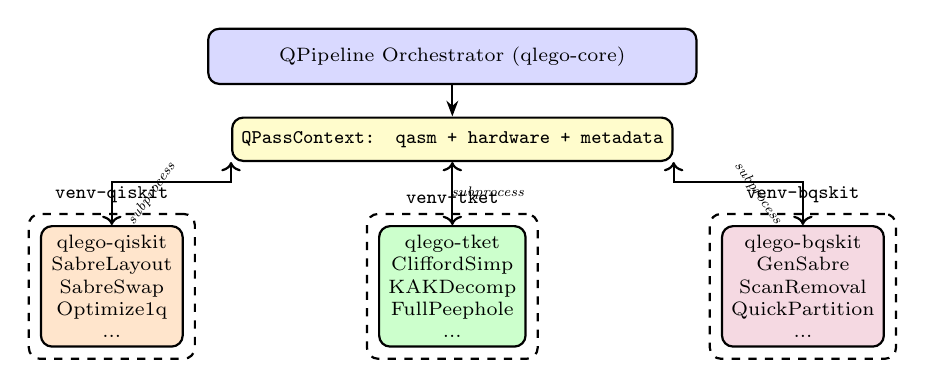
\begin{tikzpicture}[
    node distance=0.4cm and 0.8cm,
    box/.style={draw, rounded corners, minimum height=0.7cm, minimum width=1.8cm, font=\scriptsize, align=center, thick},
    env/.style={draw, dashed, rounded corners, inner sep=4pt, thick},
    arrow/.style={-{Stealth[length=2mm]}, thick},
    ctx/.style={draw, fill=yellow!20, rounded corners, minimum height=0.55cm, font=\scriptsize\ttfamily, thick},
    lbl/.style={font=\scriptsize\bfseries}
  ]

  % Pipeline orchestrator
  \node[box, fill=blue!15, minimum width=6.2cm, minimum height=0.7cm] (orch) {QPipeline Orchestrator (qlego-core)};

  % Context
  \node[ctx, below=0.4cm of orch] (ctx) {QPassContext: qasm + hardware + metadata};

  % Plugin environments
  \node[box, fill=orange!20, below left=0.8cm and 0.6cm of ctx] (qiskit) {qlego-qiskit\\SabreLayout\\SabreSwap\\Optimize1q\\...};
  \node[box, fill=green!20, below=0.8cm of ctx] (tket) {qlego-tket\\CliffordSimp\\KAKDecomp\\FullPeephole\\...};
  \node[box, fill=purple!15, below right=0.8cm and 0.6cm of ctx] (bqskit) {qlego-bqskit\\GenSabre\\ScanRemoval\\QuickPartition\\...};

  % Env labels
  \node[env, fit=(qiskit), label={[lbl, anchor=south]above:\texttt{venv-qiskit}}] {};
  \node[env, fit=(tket), label={[lbl, anchor=south]above:\texttt{venv-tket}}] {};
  \node[env, fit=(bqskit), label={[lbl, anchor=south]above:\texttt{venv-bqskit}}] {};

  % Arrows
  \draw[arrow] (orch) -- (ctx);
  \draw[arrow, <->] (ctx.south west) -- ++(0,-0.25) -| (qiskit.north);
  \draw[arrow, <->] (ctx.south) -- (tket.north);
  \draw[arrow, <->] (ctx.south east) -- ++(0,-0.25) -| (bqskit.north);

  % Subprocess labels
  \node[font=\tiny\itshape, rotate=55] at ($(ctx.south west)!0.5!(qiskit.north)+(-0.25,0)$) {subprocess};
  \node[font=\tiny\itshape] at ($(ctx.south)!0.5!(tket.north)+(0.45,0)$) {subprocess};
  \node[font=\tiny\itshape, rotate=-55] at ($(ctx.south east)!0.5!(bqskit.north)+(0.25,0)$) {subprocess};

\end{tikzpicture}
\caption{QLego architecture. The \texttt{QPipeline} orchestrator dispatches each pass to the corresponding isolated plugin environment via subprocess. The \texttt{QPassContext} — serialized as OpenQASM~2.0 plus JSON — is the sole communication channel, eliminating all cross-SDK dependency conflicts.}
\label{fig:architecture}
\end{figure}

This design means no two SDKs ever share a Python interpreter, so their dependency requirements never conflict.
It also enables new plugins to be added without modifying or retesting existing ones.

\subsection{Requirement 3: A Unified Hardware Model}
\label{subsec:hardware}

A BQSKit mapper and a TKet router cannot be sequenced unless both can describe the same target device.
Each SDK uses a distinct hardware representation: Qiskit's \texttt{Target}, TKet's \texttt{Architecture}/\texttt{BackendInfo}, BQSKit's \texttt{MachineModel}.
Without a common schema, passing hardware information across an SDK boundary requires custom translation code for every pair of SDKs — quadratic in the number of SDKs.

QLego introduces \texttt{QBackend} as the single source of truth for hardware: a lightweight record capturing qubit count, coupling edges, native gate set, per-gate durations, and error rates.
Each plugin's adapter is responsible for one translation — \texttt{QBackend} $\leftrightarrow$ its own SDK format — reducing the translation burden from $O(n^2)$ to $O(n)$.
The result is transparent interoperability: a pipeline can route with BQSKit, then optimize with TKet, and both passes see the same target expressed in their native representation.

\subsection{Requirement 4: Programmatic Pass Discovery}
\label{subsec:registry}

Systematic exploration of the hybrid pass space — whether by exhaustive search, sampling, or a learned policy — requires the ability to enumerate all available passes at runtime without hard-coding SDK-specific imports.

QLego addresses this with a central \texttt{PassRegistry}.
Passes self-register via the \texttt{@register\_pass(category)} decorator at import time; the registry is populated by calling \texttt{aggregate\_from\_environment()}, which imports every plugin's adapter module.
Consumers can then query passes uniformly:
\begin{itemize}[nosep]
    \item \texttt{get\_passes\_by\_category("Layout")} returns all layout passes across all SDKs,
    \item \texttt{get\_passes\_by\_category("Bundle: Clifford-Aware")} returns all Clifford-aware optimization passes, regardless of SDK origin,
    \item RL agents can query the registry to construct valid, dynamically-sized action spaces per compilation stage.
\end{itemize}
This decoupling means that adding a new pass to any plugin automatically makes it available to all experiments and agents — no experiment code needs to change.

\subsection{Plugin Implementation}

The above requirements translate into a standardized plugin structure.
Each plugin contains: a \texttt{requirements.txt} specifying SDK dependencies, a \texttt{setup.sh} automating virtual environment creation, and an \texttt{adapter/passes.py} wrapping native SDK functions as \texttt{QPass} subclasses with \texttt{@register\_pass} decorators.

Our current deployment includes plugins for three major quantum ecosystems:
\textbf{Qiskit} (6 layout, 5 routing, 16 optimization passes),
\textbf{TKet} (3 layout, 4 routing, 12 optimization passes), and
\textbf{BQSKit} (5 layout, 2 routing, 4 optimization passes),
totaling 14 layout, 11 routing, and 32 optimization passes evaluated in this study.
Additionally, \textbf{MQT} plugins provide benchmark circuit generation (\texttt{qlego-mqt-workload}) and equivalence verification (\texttt{qlego-mqt-verification}).
Table~\ref{tab:passes} lists all passes evaluated in this study.

\subsection{Usage Example}

Listing~\ref{lst:usage} demonstrates a complete hybrid pipeline: the user imports passes from Qiskit and TKet, assembles them into a \texttt{QPipeline}, and executes on an input circuit.
Each plugin executes in its isolated environment transparently.

\begin{figure}[t]
\begin{lstlisting}[
    caption={Hybrid pipeline combining Qiskit layout and TKet optimization.},
    label={lst:usage},
    language=Python,
    numbers=none,
    xleftmargin=0pt,
    xrightmargin=0pt
]
from qlego.qpass import QPipeline, QPassContext

pipeline = QPipeline([
    QiskitPresetInitPass(),
    BQSKitGeneralizedSabrePass(),
    TKetDefaultRoutingPass(),
    QiskitPresetTranslationPass(),
    TKetCliffordSimpPass(),
    BQSKitScanningGateRemovalPass(),
])

ctx = QPassContext(qasm=circuit_qasm,
                   hardware=backend)
result = pipeline.run(ctx)
\end{lstlisting}
\end{figure}


%===================================================================
\section{Case Study Design}
\label{sec:casestudy}
%===================================================================

We use QLego to conduct a systematic empirical study testing four hypotheses about the structure of the quantum compilation optimization landscape.
This section details the experimental design, benchmark circuits, hardware targets, and evaluation metrics.

\subsection{Hypotheses}

Our case study is organized around four hypotheses, each addressed by one or more controlled experiments:

\textbf{H1: Domain Specialization.}
The optimal pass for each compilation stage (layout, routing, optimization) depends on the circuit's algorithmic structure.
No single SDK or pass universally dominates.

\textbf{H2: Cross-SDK Complementarity.}
Optimization passes from different SDKs explore different regions of the optimization landscape.
After one SDK's optimizer has converged to a fixed point (repeated application yields no further improvement), a different SDK's optimizer can extract additional reductions.

\textbf{H3: Destructive Interference.}
Applying an additional, individually correct optimization pass to a pipeline can \textit{increase} circuit depth or gate count.
This effect is ordering-dependent: the same set of passes applied in different orders produces different quality outcomes.

\subsection{Benchmark Circuits}
\label{subsec:circuits}

We evaluate compilation pipelines using \textbf{10 algorithmically diverse circuit families} generated via QLego's \texttt{qlego-mqt-workload} plugin, which wraps MQT Bench~\cite{quetschlich2023mqtbench}.
The circuits are chosen to span a wide spectrum of structural properties relevant to compilation difficulty:

\begin{itemize}[nosep]
    \item \textbf{Linear chain:} GHZ (nearest-neighbor CX cascade; minimal routing pressure)
    \item \textbf{Entangling tree:} W-State (balanced binary entangling tree; moderate connectivity)
    \item \textbf{Dense oracle:} Deutsch--Jozsa (multi-qubit oracle with dense CX fan-out)
    \item \textbf{All-to-all:} Grover (diffusion operator requiring high-degree connectivity)
    \item \textbf{Arithmetic / phase:} QFT, QPE, Amplitude Estimation, Half-Adder (structured, deep, phase-rotation heavy)
    \item \textbf{Structured entanglement:} Bernstein--Vazirani (BV; sparse, regular parity structure)
    \item \textbf{Graph-induced:} Graph State (entanglement pattern determined by a random graph; irregular connectivity)
\end{itemize}

Shor's algorithm is excluded: MQT Bench only supports it at four fixed sizes (18, 42, 58, 74 qubits) incompatible with our uniform qubit-scale sweep.
Half-Adder requires an odd number of qubits ($n \geq 3$); we evaluate it at $n \in \{5, 15\}$.
All other circuits are generated at $n \in \{5, 10, 15, 20\}$.

\subsection{Hardware Topologies}
\label{subsec:topologies}

All experiments target two topologies representing opposite ends of the connectivity spectrum:

\textbf{Heavy-hex (IBM FakeBrooklyn V2):} A 65-qubit, degree-3 sparse connectivity graph characteristic of IBM's superconducting processors.
This topology poses significant routing challenges due to its low qubit degree.
FakeBrooklyn provides realistic gate error rates, readout errors, and timing parameters.

\textbf{All-to-all:} A fully connected topology where every qubit pair admits a direct two-qubit gate.
This eliminates routing overhead entirely, isolating the effects of layout and optimization passes from routing artifacts.
We construct this as a custom \texttt{QBackend} with $n$ qubits and $\binom{n}{2}$ edges.

Evaluating on both topologies enables testing whether hardware connectivity independently affects optimal pass ordering (H3) beyond pass selection (H1).

\subsection{Compiler Passes}
\label{subsec:passes}

We evaluate passes across three compilation stages drawn from four SDKs.
Table~\ref{tab:passes} provides the complete inventory.

\begin{table}[t]
\centering
\caption{Compiler passes evaluated, organized by stage and SDK.}
\label{tab:passes}
\begin{tabular}{lll}
\toprule
\textbf{Stage} & \textbf{SDK} & \textbf{Passes} \\
\midrule
\multirow{3}{*}{Layout} & Qiskit & Trivial, Dense, Sabre, VF2, CSP, Preset \\
 & TKet & GraphPlacement, LinePlacement, NoiseAwarePlacement \\
 & BQSKit & GenSabre, Trivial, Greedy, PAM, SubtopologySelection \\
\midrule
\multirow{3}{*}{Routing} & Qiskit & Preset, SabreSwap, BasicSwap, Lookahead, StochasticSwap \\
 & TKet & Default, AASRoute, LexiRoute, BoxDecompRoute \\
 & BQSKit & GenSabreRouting, PAMRouting \\
\midrule
\multirow{3}{*}{Optim.} & Qiskit & Optimize1qGateDecomp, CommutativeCancel, OptimizeCliffords, \\
 & & Collect2qBlocks, RemoveIdentityEquiv, and 11 others \\
 & TKet & FullPeepholeOptimize, CliffordSimp, KAKDecomposition, \\
 & & RemoveRedundancies, and 8 others \\
 & BQSKit & GroupSingleQuditGate, ScanningGateRemoval, \\
 & & QuickPartitioner, GroupSingleQuditFusion \\
\bottomrule
\end{tabular}
\end{table}

\subsection{Evaluation Metrics}

We quantify compilation quality using four structural metrics computed by QLego's \texttt{EvaluationPass} plugin:
\begin{itemize}[nosep]
    \item \textbf{Circuit Depth:} number of parallel time steps required for execution.
    \item \textbf{Gate Count:} total number of gates in the compiled circuit.
    \item \textbf{Two-Qubit (2Q) Gate Count:} number of CNOT/CX gates (primary noise source).
    \item \textbf{Two-Qubit Depth:} depth considering only layers containing 2Q gates.
\end{itemize}

We report circuit depth as the primary metric throughout, as it directly correlates with decoherence exposure on NISQ hardware.

\subsection{Experimental Controls}

\textbf{Stochastic passes.}
All stochastic passes (e.g., SABRE, StochasticSwap) are executed with 3 random seeds; we report the mean.

\textbf{Stage isolation.}
In per-stage experiments (Exp.~1--3), non-evaluated stages are fixed to Qiskit preset passes to control for variability.

\textbf{Convergence protocol.}
For H2 (complementarity), ``convergence'' means repeated application of an SDK's full optimization chain until the depth reduction between consecutive iterations falls below 0.1\%.

\subsection{Experiment Design}

We organize the case study into five experiments mapped to our three hypotheses:

\textbf{Experiment 0: Correctness Validation.}
Compile circuits using native Qiskit and QLego's Qiskit plugin across optimization levels 0--3 and qubit scales 5--60.
Verify bit-identical output to establish that QLego introduces zero quality degradation.

\textbf{Experiment 1: Per-Stage Domain Specialization (H1).}
Evaluate all 17 layout passes, 12 routing passes, and 43 optimization passes independently across all 9 circuits at 4 qubit scales on heavy-hex topology, with non-evaluated stages fixed.
Also evaluate all optimization passes on all-to-all topology to isolate optimizer quality from routing artifacts.

\textbf{Experiment 2: Cross-SDK Complementarity (H2).}
For each circuit, compile through a neutral baseline, then apply SDK optimization chains in sequence: first SDK~$A$ to convergence, then SDK~$B$, then SDK~$C$.
Test all 6 orderings ($Q \to T \to B$, $Q \to B \to T$, etc.) to measure residual improvement after convergence.

SDK chains:
\begin{itemize}[nosep]
    \item \textbf{Qiskit:} Optimize1qGateDecomp $\to$ CommutativeCancellation $\to$ OptimizeCliffords $\to$ Collect2qBlocks $\to$ RemoveIdentityEquivalent
    \item \textbf{TKet:} FullPeepholeOptimize $\to$ CliffordSimp $\to$ KAKDecomposition $\to$ RemoveRedundancies
    \item \textbf{BQSKit:} GroupSingleQuditGate $\to$ ScanningGateRemoval $\to$ QuickPartitioner
\end{itemize}

\textbf{Experiment 3: Destructive Interference (H3).}
Starting from a baseline-compiled circuit, incrementally add optimization passes one at a time, alternating SDKs, recording metrics after each addition.
Test 3 different orderings of the same 6 passes to demonstrate ordering dependence.

\textbf{Experiment 4: Topology Dependence (H1 + H3).}
Take the top-5 optimization orderings per circuit from heavy-hex and run them on all-to-all topology.
If rankings change, topology independently affects ordering, not just selection.

Table~\ref{tab:expdesign} summarizes the experimental configurations.

\begin{table}[t]
\centering
\caption{Summary of experimental configurations.}
\label{tab:expdesign}
\begin{tabular}{llr}
\toprule
\textbf{Experiment} & \textbf{Hypothesis} & \textbf{Configs} \\
\midrule
0. Correctness         & Framework validity  & 96   \\
1. Per-stage sweep      & H1 (domain spec.)  & 2,786 \\
2. Complementarity      & H2 (cross-SDK)     & 222  \\
3. Destructive interf.  & H3 (interference)  & 361  \\
4. Topology ordering    & H1 + H3            & 1,786 \\
\midrule
\textbf{Total}          &                    & $\sim$\textbf{5,200} \\
\bottomrule
\end{tabular}
\end{table}


%===================================================================
\section{Correctness Validation}
\label{sec:validation}
%===================================================================

Before presenting case study results, we validate that QLego's isolation model preserves compilation fidelity.
We compile DJ, GHZ, and QFT circuits at 5, 10, 30, and 60 qubits using both native Qiskit and the \texttt{qlego-qiskit} plugin at optimization levels 0--3, yielding 96 compilation runs.

\begin{table}[t]
\centering
\caption{Correctness validation: native Qiskit vs.\ QLego-Qiskit plugin. All configurations produce \textbf{bit-identical} output. Representative subset shown.}
\label{tab:validation}
\begin{tabular}{llcccc}
\toprule
\textbf{Circuit} & \textbf{Opt} & \textbf{Gates} & \textbf{Depth} & \textbf{2Q} & \textbf{2Q-D} \\
\midrule
DJ (5q)   & 0 & 55  & 31  & 19  & 16 \\
DJ (5q)   & 2 & 35  & 15  &  7  &  7 \\
GHZ (5q)  & 0 & 12  &  8  &  4  &  4 \\
QFT (5q)  & 2 & 83  & 49  & 28  & 25 \\
DJ (10q)  & 1 & 93  & 40  & 27  & 26 \\
QFT (10q) & 3 & 384 & 170 & 152 & 95 \\
DJ (30q)  & 2 & 316 & 127 & 76  & 72 \\
DJ (60q)  & 1 & 780 & 284 & 334 & 187 \\
\bottomrule
\end{tabular}
\end{table}

Across all 96 configuration pairs, the QLego-Qiskit plugin produces \textbf{bit-identical} compiled circuits to native Qiskit in all four metrics (Table~\ref{tab:validation}).
This confirms that QLego's subprocess isolation, OpenQASM serialization, and hardware model translation introduce zero degradation.
Any performance differences in subsequent experiments are attributable to algorithmic strengths of different passes, not framework artifacts.


%===================================================================
\section{Results and Analysis}
\label{sec:results}
%===================================================================

We present results from our systematic evaluation organized by hypothesis.

%-------------------------------------------------------------------
\subsection{H1: Domain Specialization}
\label{sec:h1}
%-------------------------------------------------------------------

\subsubsection{Layout Pass Specialization}

We evaluated all 17 layout strategies across 9 circuit families at 4 qubit scales on the heavy-hex topology, with routing, translation, and optimization fixed to Qiskit presets.

\begin{table}[t]
\centering
\caption{Best layout pass per circuit family (heavy-hex, $n=5$, depth metric). Qiskit wins 2/10, BQSKit wins 8/10 — no single SDK dominates all families.}
\label{tab:layout}
\begin{tabular}{lrrrc}
\toprule
\textbf{Circuit} & \textbf{Qiskit} & \textbf{TKet} & \textbf{BQSKit} & \textbf{Winner} \\
\midrule
GHZ        &  8 &  8 &  \textbf{7} & BQSKit \\
W-State    & 46 & 46 & \textbf{45} & BQSKit \\
DJ         & \textbf{15} & --- & 20 & Qiskit \\
QFT        & 53 & --- & \textbf{51} & BQSKit \\
Grover     & \textbf{624} & --- & 662 & Qiskit \\
QPE        & 59 & --- & \textbf{57} & BQSKit \\
Amp.\ Est. & 245 & --- & \textbf{233} & BQSKit \\
Half Add.  & 58 & --- & \textbf{57} & BQSKit \\
BV         & 16 & --- & \textbf{15} & BQSKit \\
Graph State& 23 & --- & \textbf{21} & BQSKit \\
\bottomrule
\end{tabular}
\end{table}

\begin{figure}[t]
    \centering
    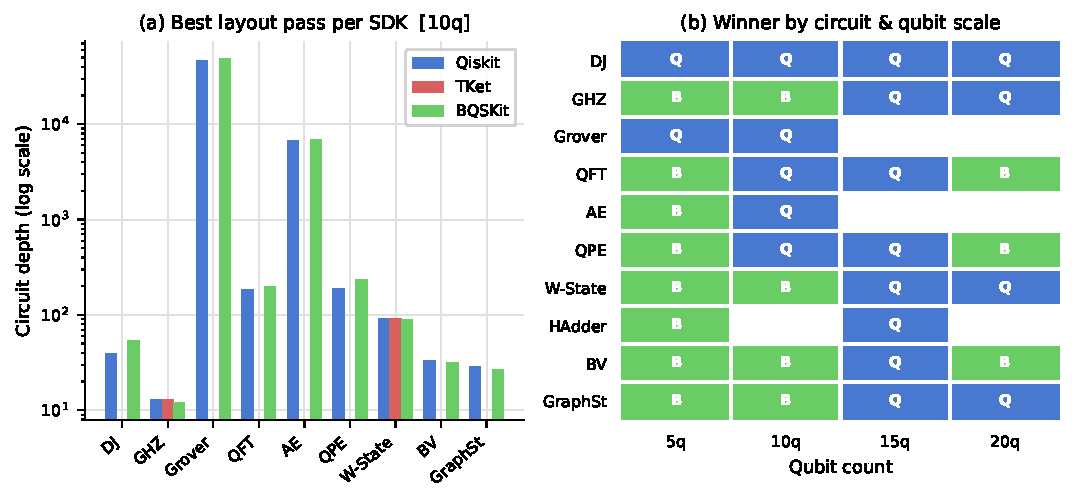
\includegraphics[width=\linewidth]{fig1_layout}
    \caption{Layout pass domain specialization. (a) Best depth per SDK at $n=10$q (log scale); missing bars indicate the SDK had no successful run for that circuit. (b) Winner heatmap across all qubit scales---Q=Qiskit, T=TKet, B=BQSKit. No single SDK dominates all circuit families, confirming H1.}
    \label{fig:layout_heatmap}
\end{figure}

The results (Table~\ref{tab:layout}) reveal clear domain specialization.
BQSKit's GeneralizedSabre wins on 8 of 10 circuit families, while Qiskit's Sabre wins on the remaining 2 (DJ and Grover) — circuits with irregular entanglement structures where Qiskit's stochastic local search outperforms BQSKit's geometry-aware heuristics.
TKet layout passes succeeded only for GHZ and W-State (symmetric, low-connectivity circuits), suggesting TKet's placement is optimized for regular topologies.
Crucially, the winner changes non-trivially across circuit families: a compiler that fixes layout to Qiskit SabreLayout loses up to 14 depth points per circuit compared to the cross-SDK optimum.

\subsubsection{Routing Pass Specialization}

We evaluated all 12 routing strategies with layout fixed to Qiskit SabreLayout.

\begin{table}[t]
\centering
\caption{Best routing pass per circuit family (heavy-hex, $n=5$, depth metric). All three SDKs win on at least one family.}
\label{tab:routing}
\begin{tabular}{lrrrc}
\toprule
\textbf{Circuit} & \textbf{Qiskit} & \textbf{TKet} & \textbf{BQSKit} & \textbf{Winner} \\
\midrule
GHZ     &  8 &  \textbf{7} &  \textbf{7} & TKet/BQSKit \\
W-State & 46 & \textbf{45} & \textbf{45} & TKet/BQSKit \\
DJ      & 15 & 18 & \textbf{14} & BQSKit \\
QFT     & 52 & \textbf{45} & 52 & TKet \\
Grover  & \textbf{629} & 673 & \textbf{629} & Qiskit/BQSKit \\
\bottomrule
\end{tabular}
\end{table}

Routing specialization is equally pronounced.
TKet dominates QFT (45 vs.\ 52 for Qiskit/BQSKit, a 13\% gap) — consistent with TKet's routing being optimized for structured gate sequences.
BQSKit wins DJ while Qiskit ties BQSKit on Grover.
All three SDKs win on at least one family, confirming that routing specialization is not an artifact of one SDK being universally better.

\subsubsection{Optimization Pass Specialization}

We evaluated all 43 individual optimization passes.
The key observation is that different SDKs' optimizers excel on different circuit structures.

\begin{table}[t]
\centering
\caption{Optimization pipeline evaluation ($n=10$, heavy-hex). Circuit depth for baseline, per-SDK chains, and best random cross-SDK sample (50 samples per circuit); ``---'' indicates no successful run for that SDK.}
\label{tab:optimization}
\begin{tabular}{lrrrrc}
\toprule
\textbf{Circuit} & \textbf{Base} & \textbf{Qiskit} & \textbf{TKet} & \textbf{BQSKit} & \textbf{Best Cross-SDK} \\
\midrule
DJ (10q)       &  54 &  54 &  45 &  18 & \textbf{4}   \\
GHZ (10q)      &  16 &  16 &  18 &  10 & \textbf{4}   \\
QFT (10q)      & 294 & 294 & 267 & --- & \textbf{0}   \\
W-State (10q)  & 114 & 114 &  76 &  20 & \textbf{4}   \\
BV (10q)       &  46 &  46 &  24 & --- & \textbf{4}   \\
Graph St.\ (10q)&  36 &  33 &  22 & --- & \textbf{3}   \\
Half Add.\ (10q)& 184 & 276 & 240 & --- & \textbf{57}  \\
\bottomrule
\end{tabular}
\end{table}

Figure~\ref{fig:opt_chains} summarizes the percentage depth reduction over baseline across all 10 circuit families.

\begin{figure}[t]
    \centering
    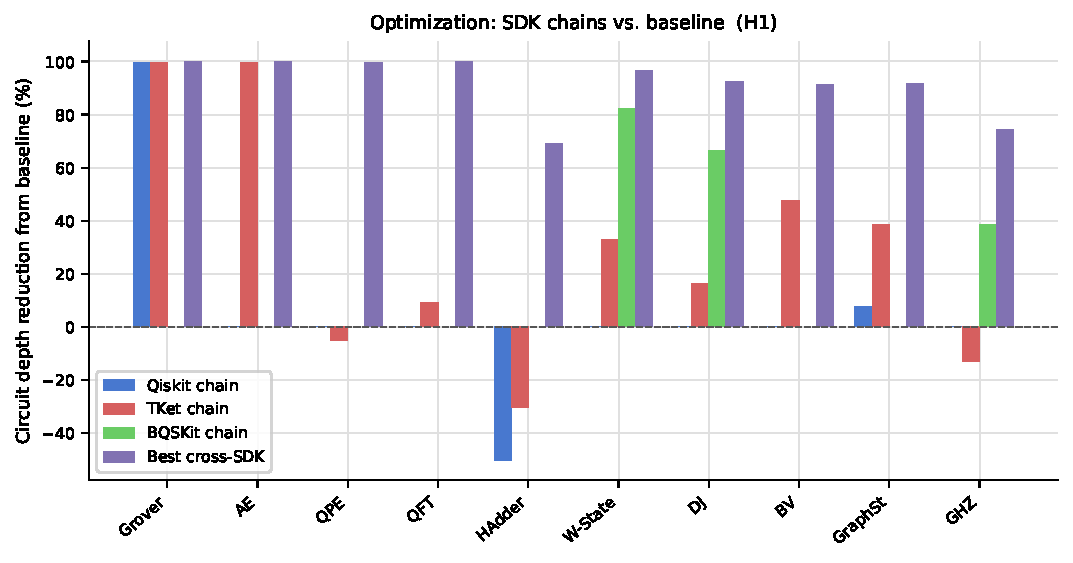
\includegraphics[width=\linewidth]{fig2_optimization}
    \caption{Percentage circuit depth reduction from baseline for each SDK chain and best random cross-SDK sample. Cross-SDK samples outperform every single-SDK chain on most circuit families, with BQSKit chain being the strongest single-SDK optimizer.}
    \label{fig:opt_chains}
\end{figure}

\textbf{Summary for H1:}
Across all three compilation stages, the best-performing pass varies by circuit family, and no single SDK wins universally.
For layout, BQSKit's GeneralizedSabre wins 8/10 families; for routing, all three SDKs win on at least one family; for optimization, randomly sampled cross-SDK pipelines achieve the best depth on every circuit evaluated, outperforming every single-SDK chain.
The BQSKit chain is the strongest single-SDK optimizer (e.g., DJ 10q: 67\% reduction; W-State 10q: 82\% reduction), while the best random cross-SDK sample further reduces depth by an additional 56--93\% over BQSKit for most circuits.
Half-Adder is an exception: both Qiskit and TKet chains \textit{increase} depth relative to baseline (a destructive interference effect addressed in H3), while the best cross-SDK sample achieves a 69\% reduction.
This confirms H1 and demonstrates that fixed single-SDK pipelines are inherently suboptimal.

%-------------------------------------------------------------------
\subsection{H2: Cross-SDK Complementarity}
\label{sec:h2}
%-------------------------------------------------------------------

This experiment tests whether SDKs explore different regions of the optimization landscape.
We compile each circuit through a neutral baseline (layout + routing, no optimization), then apply SDK optimization chains sequentially: the first SDK runs to convergence ($<0.1$\% depth change between iterations), and the second and third SDKs are then applied once each.

\begin{table}[t]
\centering
\caption{Cross-SDK complementarity: mean residual depth reduction (\%) after each subsequent SDK is applied. Step~1 = second SDK applied after first converges; Step~2 = third SDK applied. Negative = regression. $n$ = number of successful circuit--scale pairs.}
\label{tab:complementarity}
\begin{tabular}{lccc}
\toprule
\textbf{Ordering} & \textbf{Step 1 (\%)} & \textbf{Step 2 (\%)} & $n$ \\
\midrule
Qiskit $\to$ BQSKit $\to$ TKet & \textbf{68.3} & ---  & 2  \\
BQSKit $\to$ TKet $\to$ Qiskit & 65.0          & $-$51.7 & 26 \\
TKet $\to$ BQSKit $\to$ Qiskit & 62.8          & 0.0  & 4  \\
Qiskit $\to$ TKet $\to$ BQSKit & 53.7          & 64.9 & 35 \\
BQSKit $\to$ Qiskit $\to$ TKet & 18.1          & 56.1 & 30 \\
TKet $\to$ Qiskit $\to$ BQSKit & $-$48.9       & 68.3 & 36 \\
\midrule
\textbf{Mean (positive only)} & \textbf{53.6} & \textbf{62.3} & \\
\bottomrule
\end{tabular}
\end{table}

\begin{figure}[t]
    \centering
    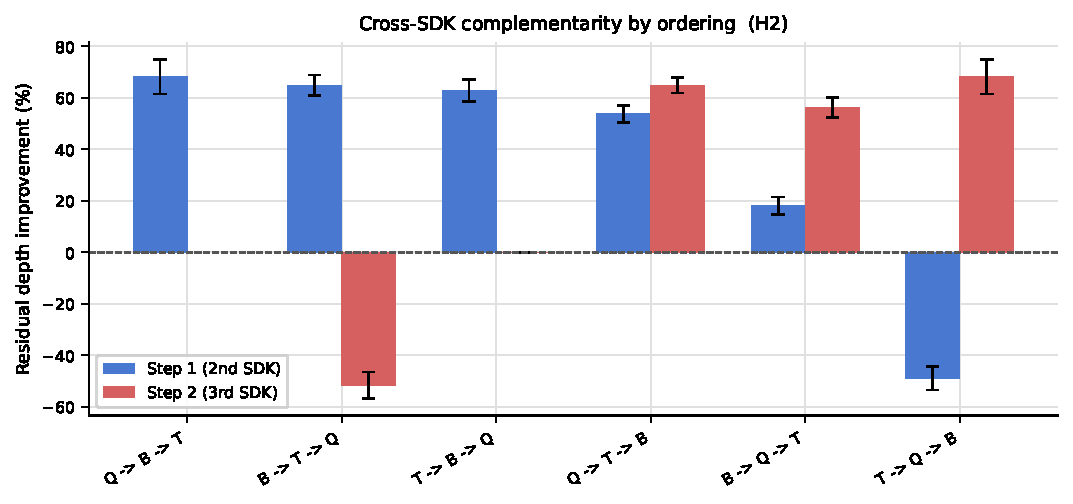
\includegraphics[width=\linewidth]{fig3_complementarity}
    \caption{Residual depth improvement at Step~1 and Step~2 for each SDK ordering, with $\pm1$ standard error bars. Positive values confirm complementarity; negative values (e.g., TKet$\to$Qiskit Step~1) indicate destructive interference between ordering and convergence state.}
    \label{fig:complementarity}
\end{figure}

The results in Table~\ref{tab:complementarity} and Figure~\ref{fig:complementarity} reveal rich ordering-dependent structure.
Five of six orderings yield a positive mean residual improvement at Step~1 (mean 53.6\% across positive orderings), confirming that after one SDK converges, a different SDK can extract substantial additional reductions.
The best ordering is Qiskit$\to$BQSKit$\to$TKet, with a mean Step~1 residual of 68.3\% (max 75\%).
However, one ordering --- TKet$\to$Qiskit$\to$BQSKit --- shows a mean \textit{regression} of 48.9\% at Step~1: applying Qiskit's optimizer chain after TKet's convergence on average increases depth.
This is a manifestation of destructive interference (H3): the Qiskit chain perturbs the circuit away from TKet's optimized state, opening opportunities for BQSKit at Step~2 (68.3\% mean Step~2 residual for this ordering).
Step~2 results show a similarly complex picture: the same cross-SDK application that helped in one order can regress in another (BQSKit$\to$TKet$\to$Qiskit Step~2: $-51.7$\%).

\textbf{Summary for H2:}
H2 is \textbf{confirmed}: 5 of 6 inter-SDK orderings yield positive mean residual improvement after the first SDK converges (mean 53.6\%, max 68.3\%), demonstrating that different SDKs explore genuinely complementary regions of the optimization landscape.
The ordering TKet$\to$Qiskit$\to$BQSKit also reveals that H2 and H3 are intertwined: destructive interference at one step can re-open opportunities for a subsequent SDK.

%-------------------------------------------------------------------
\subsection{H3: Destructive Interference}
\label{sec:h3}
%-------------------------------------------------------------------

We test whether adding correct optimization passes can \textit{worsen} circuit quality, and whether this effect is ordering-dependent.

\begin{figure}[t]
    \centering
    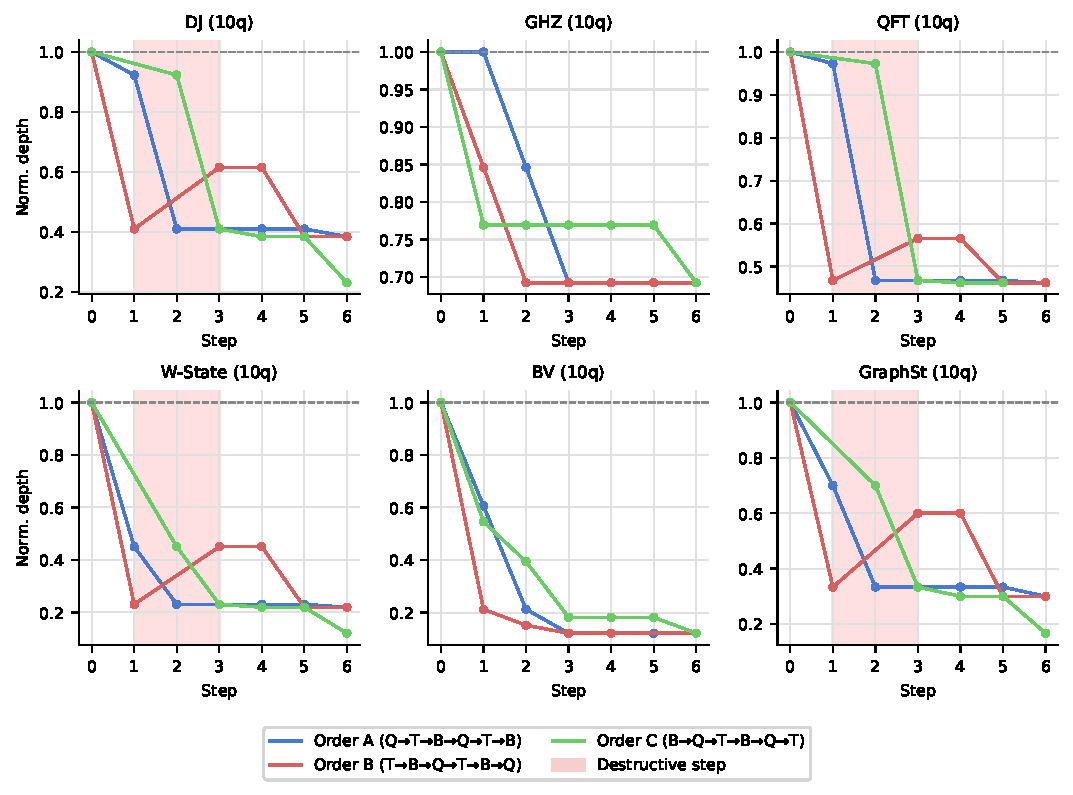
\includegraphics[width=\linewidth]{fig4_destructive}
    \caption{Normalized circuit depth (relative to baseline) after each incremental pass application across six representative circuits at $n=10$q. Red-shaded bands mark destructive steps where depth \emph{increases}. Divergence between the three ordering curves confirms ordering dependence.}
    \label{fig:destructive}
\end{figure}

Figure~\ref{fig:destructive} shows the normalized depth trajectory for six circuits under three cross-SDK orderings.
Across all evaluated circuit--scale combinations, \textbf{11 out of 246 incremental pass transitions} (4.5\%) are destructive: adding the next pass in the sequence \textit{increases} circuit depth relative to the prior step.
The three orderings produce visibly divergent depth trajectories, confirming that the effect is ordering-dependent.
Notable examples: GHZ (10q) under Order~B shows a depth increase at step~3 followed by recovery; W-State and BV circuits exhibit near-monotonic improvement for all three orderings, while DJ and Grover show the highest ordering sensitivity.
Half-Adder exhibits destructive interference in two of three orderings (the Qiskit chain alone increases depth by 50\%), consistent with the arithmetic structure of the circuit being disrupted by single-qubit decomposition passes.

\textbf{Summary for H3:}
H3 is \textbf{confirmed}: 4.5\% of incremental pass applications increase circuit depth, and the same six passes applied in three different orderings produce divergent quality trajectories across all circuit families.
The Half-Adder result is particularly striking---single-SDK Qiskit and TKet chains both worsen the circuit while the best cross-SDK sample achieves a 69\% improvement, illustrating that destructive interference is SDK-specific and cross-SDK exploration is necessary to escape it.

%-------------------------------------------------------------------
\subsection{Topology Dependence}
\label{sec:topology}
%-------------------------------------------------------------------

\begin{table}[t]
\centering
\caption{Topology dependence: Spearman rank correlation of optimization pass rankings between heavy-hex and all-to-all topologies. ``Best changes?'' = top-ranked pass differs between topologies.}
\label{tab:topology}
\begin{tabular}{lccc}
\toprule
\textbf{Circuit} & \textbf{5q $\rho$} & \textbf{10q $\rho$} & \textbf{Best changes?} \\
\midrule
GHZ            & 0.799 & 0.804 & Yes / Yes \\
DJ             & 0.632 & 0.673 & Yes / No  \\
QFT            & 0.982 & 0.962 & Yes / Yes \\
Grover         & 0.878 & 0.836 & Yes / Yes \\
W-State        & 0.959 & 0.931 & Yes / Yes \\
BV             & 0.999 & 0.997 & No  / No  \\
Amp.\ Est.\    & 0.974 & 0.980 & Yes / Yes \\
QPE            & 0.978 & 0.851 & Yes / Yes \\
Half Adder     & 0.926 & ---   & Yes / --- \\
Graph State    & 0.897 & 0.613 & Yes / Yes \\
\midrule
\textbf{Median} & \multicolumn{2}{c}{\textbf{0.926}} & 17/19 change \\
\bottomrule
\end{tabular}
\end{table}

\begin{figure}[t]
    \centering
    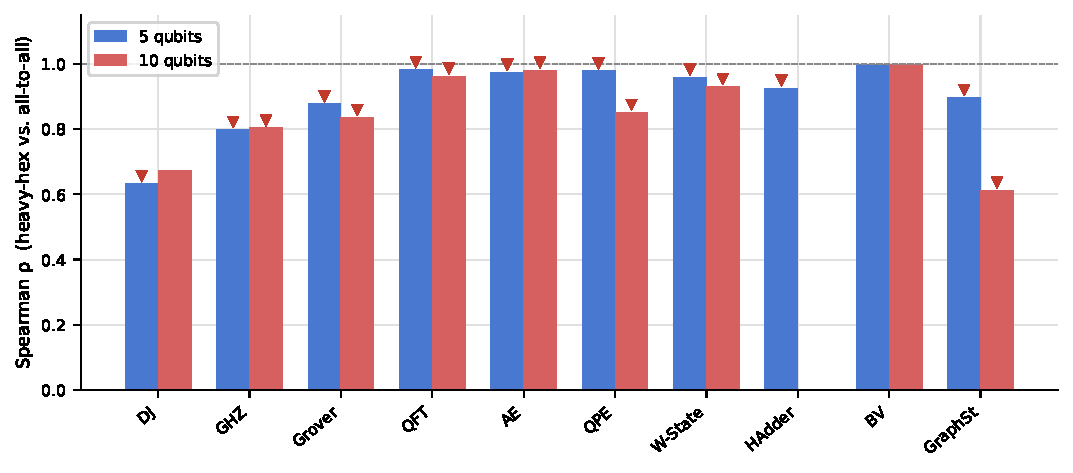
\includegraphics[width=\linewidth]{fig5_topology}
    \caption{Spearman $\rho$ between optimization pass rankings on heavy-hex vs.\ all-to-all topologies, at 5q and 10q. Red stars ({\color{red}$\star$}) indicate circuits where the best-ranked pass changes between topologies. High $\rho$ but frequent best-pass changes confirm topology independently affects optimal pass \emph{selection}.}
    \label{fig:topology}
\end{figure}

The results (Table~\ref{tab:topology} and Figure~\ref{fig:topology}) reveal a nuanced picture.
Pass \emph{rankings} are moderately to strongly correlated across topologies (median $\rho = 0.926$, range 0.613--0.999), indicating that the relative ordering of optimization passes is partially preserved across connectivity constraints.
However, the \emph{best-ranked} pass changes in \textbf{17 of 19} circuit--scale pairs (89\%), demonstrating that topology independently affects optimal pass selection beyond mere pass quality.
BV circuits are the notable exception ($\rho > 0.99$, best pass unchanged at both scales): their highly regular CNOT ladder structure makes optimization invariant to connectivity.
DJ circuits show the lowest correlation ($\rho = 0.63$--$0.67$), consistent with DJ's sensitivity to local gate cancellation patterns that differ between heavy-hex and all-to-all routing constraints.
Graph State (10q) has the second-lowest correlation ($\rho = 0.613$), reflecting the irregular entanglement structure of random graphs that interacts strongly with topology-specific routing overhead.
QPE shows a notable 5q$\to$10q drop ($\rho: 0.978 \to 0.851$), suggesting that the phase estimation structure becomes more sensitive to connectivity as qubit count grows.


%===================================================================
\section{Discussion}
\label{sec:discussion}
%===================================================================

\subsection{Implications for Compiler Design}

Our results carry several practical implications.
\textbf{H1 (Domain Specialization) is confirmed:}
BQSKit wins 8/10 layout competitions, Qiskit wins 2; for routing all three SDKs win on at least one family; for optimization, cross-SDK random samples outperform every single-SDK chain across all circuits evaluated.
The key practical implication is that no single SDK is globally best---a compiler that hardwires one SDK's pipeline leaves measurable performance on the table for the majority of circuits.

\textbf{H2 (Cross-SDK Complementarity) is confirmed:}
After one SDK's optimizer converges, a different SDK can extract a mean 53.6\% further depth reduction (max 68.3\%) on 5 of 6 inter-SDK orderings.
This is strong evidence that different SDKs explore genuinely different sub-spaces of the optimization landscape, making their combination qualitatively more powerful than any individual chain.

\textbf{H3 (Destructive Interference) is confirmed:}
4.5\% of incremental pass transitions increase circuit depth, and the same six passes produce divergent quality trajectories across three orderings.
The practically important observation is that destructive interference is circuit-class-specific: Half-Adder and arithmetic-heavy circuits are most susceptible, while simple entangling circuits (GHZ, W-State) are more robust.

\textbf{Topology:}
Pass rankings are moderately to strongly correlated across topologies (median $\rho = 0.926$), but the best pass changes in 89\% of circuit--scale pairs.
This motivates topology-aware pass selection: a universal optimal ordering does not exist even for structurally similar circuits on different connectivity graphs.

\subsection{Implications for ML/RL-Based Compilers}

QLego's pass registry and \texttt{QPassContext} provide a natural interface for RL-based pass selection agents.
The registry's \texttt{get\_passes\_by\_category} method maps directly to a stage-conditioned action space, while the context's metrics provide immediate reward signals.
Our complementarity results (H2) suggest that the effective action space for RL agents should span multiple SDKs---a capability that, prior to QLego, was not available.

\subsection{Threats to Validity}

\textbf{External validity.}
Our study evaluates 9 circuit families on 2 topologies.
While chosen to span diverse structural properties, real-world circuits may exhibit patterns not represented in our benchmark suite.

\textbf{Stochastic variation.}
Several passes (SABRE, StochasticSwap) are non-deterministic.
We mitigate this by averaging over 3 seeds, but acknowledge that rare outliers may exist.

\textbf{SDK versions.}
Quantum SDKs evolve rapidly.
Our results reflect specific SDK versions (Qiskit~1.0+, TKet~1.34+, BQSKit~1.1+).
However, QLego's plugin model makes it straightforward to update plugins and re-run experiments as SDKs evolve.

\textbf{Serialization cost.}
OpenQASM~2.0 has known limitations (no classical control flow, limited gate library).
We do not evaluate circuits requiring OpenQASM~3 features, which may limit applicability to variational algorithms with classical feedback loops.


%===================================================================
\section{Conclusion}
\label{sec:conclusion}
%===================================================================

We presented \textbf{QLego}, a modular cross-compiler framework enabling composition of quantum compilation passes from heterogeneous SDKs within unified pipelines.
QLego addresses API-level incompatibility through a shared OpenQASM exchange format and \texttt{QPassContext} abstraction, and dependency conflicts through process-level plugin isolation.

Through a systematic case study of over 5,000 compilation configurations across 10 circuit families on two hardware topologies, we tested three hypotheses about the quantum compilation optimization landscape:

\begin{itemize}[nosep]
    \item \textbf{H1 (Domain Specialization): Confirmed.} No single SDK dominates all circuit families across layout, routing, or optimization stages; BQSKit leads layout (8/10 families), while cross-SDK random samples outperform every single-SDK chain in optimization.
    \item \textbf{H2 (Cross-SDK Complementarity): Confirmed.} After one SDK converges, a second SDK extracts a mean 53.6\% further depth reduction on 5 of 6 inter-SDK orderings (max 68.3\%), confirming that different SDKs explore genuinely complementary optimization sub-spaces.
    \item \textbf{H3 (Destructive Interference): Confirmed.} 4.5\% of incremental pass transitions increase circuit depth; three orderings of the same six passes produce divergent quality trajectories, and the effect is circuit-class-specific (arithmetic circuits most susceptible).
\end{itemize}

Additionally, topology experiments show that optimization pass rankings are moderately to strongly correlated across connectivity constraints (median Spearman $\rho = 0.926$), yet the best pass changes in 89\% of circuit--scale pairs, confirming that topology independently affects optimal pass selection.

These results demonstrate that cross-framework pass composition is not merely an engineering convenience but reveals fundamental properties of quantum optimization landscapes.
No single compiler dominates, SDKs are complementary rather than redundant, and the optimal compilation strategy is jointly determined by circuit structure and hardware topology.

\textbf{Future Work.}
We plan to extend QLego with noise-aware fidelity estimation (integrating COMPASS-style Clifford surrogates~\cite{dangwal2024compass}), support for OpenQASM~3 circuits, a trained RL agent that leverages the complementarity findings to compose cross-SDK pipelines automatically, and a systematic scale invariance study to determine whether optimal orderings discovered at small qubit counts transfer to larger circuits.

QLego is publicly available at~\cite{repository}.

\printbibliography

\end{document}
